\subsection{Flankengetriggertes D-Latch} % (fold)
\label{sub:Flankengetriggertes D-Latch}
\begin{frame}
    \frametitle{Flankengetriggertes D-Latch}
    \framesubtitle{}
     \begin{figure}[H]
     \begin{center}
             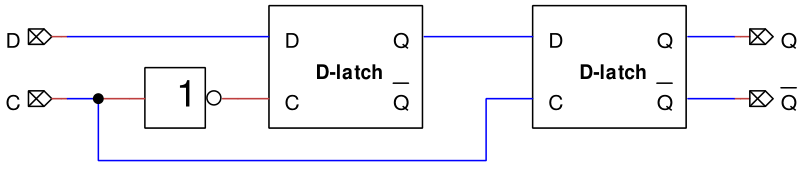
\includegraphics[scale=0.3]{./img/schaltung/flanken_d.png}
     \end{center}
     \end{figure}
\end{frame}
\begin{frame}
    \frametitle{Flankengetriggertes D-Latch}
    \framesubtitle{}
     \begin{columns}[c]
         \column{0.6\textwidth}
         \begin{figure}[H]
         \begin{center}
                 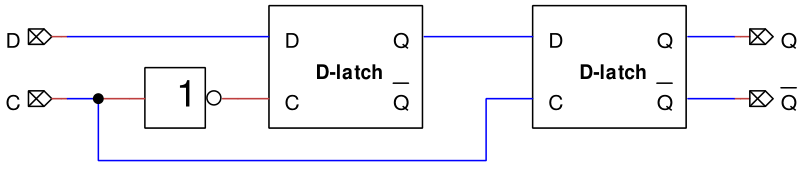
\includegraphics[scale=0.25]{./img/schaltung/flanken_d.png}
         \end{center}
         \end{figure}
         \column{0.4\textwidth}
         \begin{figure}[H]
         \begin{center}
                 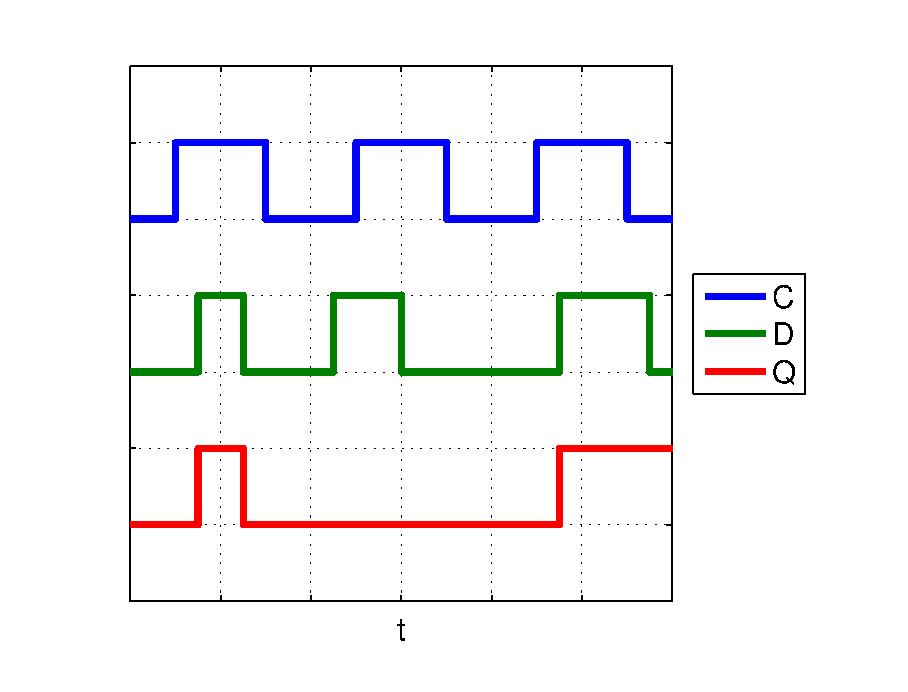
\includegraphics[scale=0.3]{./img/Aufgabe_3_d.eps}
         \end{center}
         \end{figure}
     \end{columns}
     \begin{block}{Funktionsweise}
        \begin{itemize}
            \item Clock muss vor Triggerung auf 1 stehen 
            \item Flanken werden nicht erkannt
        \end{itemize}
     \end{block}
\end{frame}
% subsection Flankengetriggertes D-Latch (end)
